\documentclass[tikz,border=2pt]{standalone}
\usepackage{amsmath,amssymb}
\usetikzlibrary{arrows.meta}
\begin{document}
% Two machines, one mechanic: lambda(0) = 2, lambda(1) = 1 (failures, blue), mu(1) = mu(2) = 2
% (repairs, red). Level crossing: 2 p(0) = 2 p(1), 1 p(1) = 2 p(2); p = (0.4, 0.4, 0.2).
% Flows across the cuts: 0.8 and 0.4.
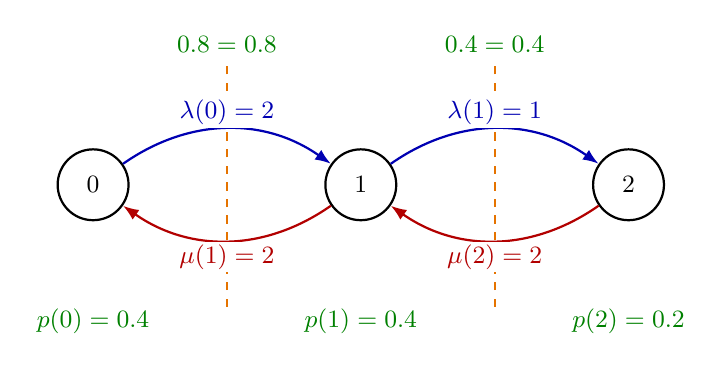
\begin{tikzpicture}[font=\small, >={Latex[length=2mm]},
    st/.style={circle, draw, thick, minimum size=9mm, inner sep=1pt}]
  \node[st] (s0) at (0,0) {$0$};
  \node[st] (s1) at (3.4,0) {$1$};
  \node[st] (s2) at (6.8,0) {$2$};
  % cuts
  \draw[orange!90!black, thick, dashed] (1.7,-1.55) -- (1.7,1.55);
  \draw[orange!90!black, thick, dashed] (5.1,-1.55) -- (5.1,1.55);
  % arrivals (failures)
  \draw[->, blue!70!black, thick] (s0) to[bend left=35] node[above, fill=white, inner sep=1pt] {$\lambda(0)=2$} (s1);
  \draw[->, blue!70!black, thick] (s1) to[bend left=35] node[above, fill=white, inner sep=1pt] {$\lambda(1)=1$} (s2);
  % departures (repairs)
  \draw[->, red!70!black, thick] (s1) to[bend left=35] node[below, fill=white, inner sep=1pt] {$\mu(1)=2$} (s0);
  \draw[->, red!70!black, thick] (s2) to[bend left=35] node[below, fill=white, inner sep=1pt] {$\mu(2)=2$} (s1);
  \node[green!50!black, anchor=south] at (1.7,1.55) {$0.8=0.8$};
  \node[green!50!black, anchor=south] at (5.1,1.55) {$0.4=0.4$};
  % time-average probabilities
  \node[green!50!black, anchor=north] at (0,-1.45) {$p(0)=0.4$};
  \node[green!50!black, anchor=north] at (3.4,-1.45) {$p(1)=0.4$};
  \node[green!50!black, anchor=north] at (6.8,-1.45) {$p(2)=0.2$};
\end{tikzpicture}
\end{document}
